\documentclass[12pt]{article}
\usepackage{hyperref}
\usepackage[pdftex]{graphicx}
\usepackage{multirow}
\usepackage{setspace}
\usepackage{color}
\usepackage{multicol}

% Tennessee Technological University
% ME4140 - Fall 2016 - Fall2017 - Fall 2020 
% Tristan Hill - August 08, 2020

\textwidth=6.5in
\topmargin=-0.5in
\textheight=9.25in
\hoffset=-0.5in
\footskip=0.2in

\pagestyle{myheadings}
\markright{{\large ME 4140 Fall 2019---The Robotic Operating System}}

\newcommand{\homeWeight}{10}
\newcommand{\quizWeight}{20}
\newcommand{\examWeight}{15}
\newcommand{\finalWeight}{25}

\begin{document}

\thispagestyle{plain}

\begin{center}
    {\bf \Large ROS - The Robotic Operating System} \vspace{3mm} \\
   {\bf \large ME 4140 - Introduction to Robotics - Fall 2020} \\
\end{center}

\Large
\begin{description}

    	\item[What is ROS?]: 
            \begin{enumerate}
		\item {\it The Robot Operating System (ROS) is a flexible framework for writing robot software. It is a collection of tools, libraries, and conventions that aim to simplify the task of creating complex and robust robot behavior across a wide variety of robotic platforms.} - \href{http://www.ros.org/about-ros/}{ROS}       
                 \item Software Framework for Robotics Development
                \item {\it not} what you may think when you hear {\it operating system}                    
            \end{enumerate}
      
        \item[What are the benefits of using ROS?]: 
            \begin{enumerate}
                \item Hardware/Software Compatibility   
                \item Multi-threading, Parallel Processing, Distributed Computing  
                \item Open Source Community (BSD)    
                \item High Level Robotics Development                   
            \end{enumerate}    
            
%        \item[Who is using ROS?]:
%             \begin{enumerate}
%                \item Researchers  
%                \item Students    
%                \item Industry - {\it start ups} and {\it big business (?)}                  
%            \end{enumerate} 

        \item[Where did ROS come from?]:
            \begin{enumerate}
                \item Originally developed at Stanford (mid 2000s)
                \item Continued by Willow Garage (2007)
                \item Maintained by an international community of open source developers (present)
                \item {\it The ROS ecosystem now consists of tens of thousands of users worldwide, working in domains ranging from tabletop hobby projects to large industrial automation systems.} - \href{http://www.ros.org/history/}{ROS}
            \end{enumerate} 

            \newpage
            
            \item [How Does it Work?]:
            \begin{enumerate}
                \item ROS is based on a system of connected {\it nodes} 
                \item Each node represents a different element in the robotic system
                   
                   \begin{itemize}
                        \item Laser
                        \item Drive Kinematics
                        \item Navigation
                        \item Manipulator
                        \item etc.
                    \end{itemize}
                \vspace{15mm}
                \item Each node can have corresponding source code, executables, and data files.\\
\item Software Languages
                \begin{itemize}
                \item C++ 
                \item Python
                \item {\it markup languages} such as XML and YAML\\
                 \end{itemize}
                 
                \item Nodes communicate or share information in  different ways. 
                 \begin{itemize}
                        \item Topics - {\it publish} and {\it subscribe} to specific information.
                        \item Parameter Server - Static Data
                        \item Services - RPC - Single Request \\\\
                    \end{itemize} 
                
                \item The parallel processing and message passing is handled by ROS. Distributed computing is supported for off board computing and multi-robot applications.
            \end{enumerate}    
         
         \newpage
         \item [Supprted Robots]:\\
                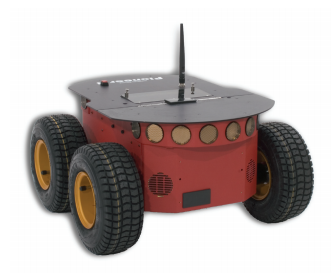
\includegraphics[scale=1]{p3at.PNG}
            

                
            \newpage
            \textbf{ Videos:} \\\\
       \href{https://youtu.be/wXPLH_2IRVw}{Turtlebot}\\\\
                \href{https://www.dropbox.com/s/adpg9v3lvfltd92/lx_demo_cut_07_07_2020.mp4?dl=0}{Pinoeer LX}\\\\

                \href{https://youtu.be/lcICvz5jMHw}{Aubo Arm}\\

%            \item [How to get Started!]: There are several ways to get started but it is recommended that you use Ubuntu 16 LTS. ROS is also available for Ubuntu 18 LTS. There has also been talk of ROS on windows. 
%                \begin{enumerate}
%                    \item Install Ubuntu - 3 options
%                        \begin{enumerate}
%                            \item Virtualize Ubuntu with {\it Virtual Box}
%                            \item Install Ubuntu permanently on your machine {\it True Boot}
%                            \item Run Ubuntu temporarily on your machine {\it wubi.exe boot}        
%                        \end{enumerate}
%                    
%                    \item Install ROS Indigo
%                        \begin{enumerate}
%                            \item before you change your linux system it is a good idea to back it up!
%                            \item make sure your system can connect to the internet
%                            \item check that your system can successfully update (not upgrade OS)
%                            \item in a terminal \$sudo apt-get check , you  will be prompted for the administrator password and if you do not see any errors you are ready to go!      
%                        \end{enumerate}
%                    
%                \end{enumerate}
                    
         
            
\end{description}


\end{document}

